% Chapter 1

\chapter{Prototype II} % Main chapter title

\label{prototytpe2chapter} % For referencing the chapter elsewhere, use \ref{Chapter1} 

\lhead{Chapter \emph{Prototype II}} % This is for the header on each page - perhaps a shortened title

%----------------------------------------------------------------------------------------
\section{Prototype Development Iteration II}
I started the next iteration of prototype development that aimed to improve the first prototype described in the chapter \ref{prototype1chapter}. In the second prototype the emphasis was more on improving support for the three psychological needs from self-determination theory \citep{ryan2000:self} which are relatedness, competence, and autonomy. I substituted Facebook social plugins with features that could allow users to directly comment on or like each other. Facebook social plugins failed to integrate seamlessly with the app since the network signal was a bit poor in the area where I conducted experiments, therefore users failed to load them into the app. In addition, the system comprised SMS reminders and feedbacks instead of Facebook based reminders. The new system (Figure \ref{figure:prototype_2_screens} ) had the following features of which most of them were improvements from the previous prototype:
\begin{enumerate}
\item{Recording of meals} consumed by a beneficiary user.
\item{A pedometer} for detection of steps walked by beneficiary user.
\item{Pie charts} that show summaries of food groups consumed by a beneficiary user.
\item{Bar charts} that show steps walked by a beneficiary user (daily intervals, 7 days intervals, and, weeks of a month intervals).
\item{Avatars} that can be changed in order to increase autonomy of intermediary users.
\item{Badges} that can be earned through a combination of steps walked by a beneficiary participant and the number of days they app has been utilized by a pair of users. In the previous prototype it was easier to jump from the lowest badge to the highest without passing through intermediate badges as longer as a pair had enough clicks. Therefore, to move to a higher badge in this second prototype a pair was required to use an app for a certain number of days and then couldn't by [ass any badge as the process was incremental. To reach the highest badges pairs were required to pass through all the badges in between in different days, and also to meet requirements for the King/Queen badge which were at least an average of ten thousand (10000) steps walked by a beneficiary user in a day, and at least 18 days of usage activity detected from the app. 
\item{Score board/ leader board} of which points were earned by averaging between points scored from usage (i.e each day of usage resulted into 1000 points earned) and points earned as the result of beneficiary's average number of steps walked (i.e. if the average is \emph{n} steps/day then the number of points accumulated is ``n'')
\item{Botanical gardens} that consisted of trees and flowers. Trees on the garden grows proportional with badges while flowers grows proportionally with number of meals recorded. if a recorded meal contains fruits and vegetables it is an added advantage.
\item{Fish tanks or bowls / Aquarium} that consisted of Fish of different species. Number of species grows proportional with badges while the size of each specie is proportional to number of meals recorded. If a recorded meal contains fruits and vegetables it is an added advantage on the size.
\end{enumerate}
\begin{figure}[htbp]
  \centering
    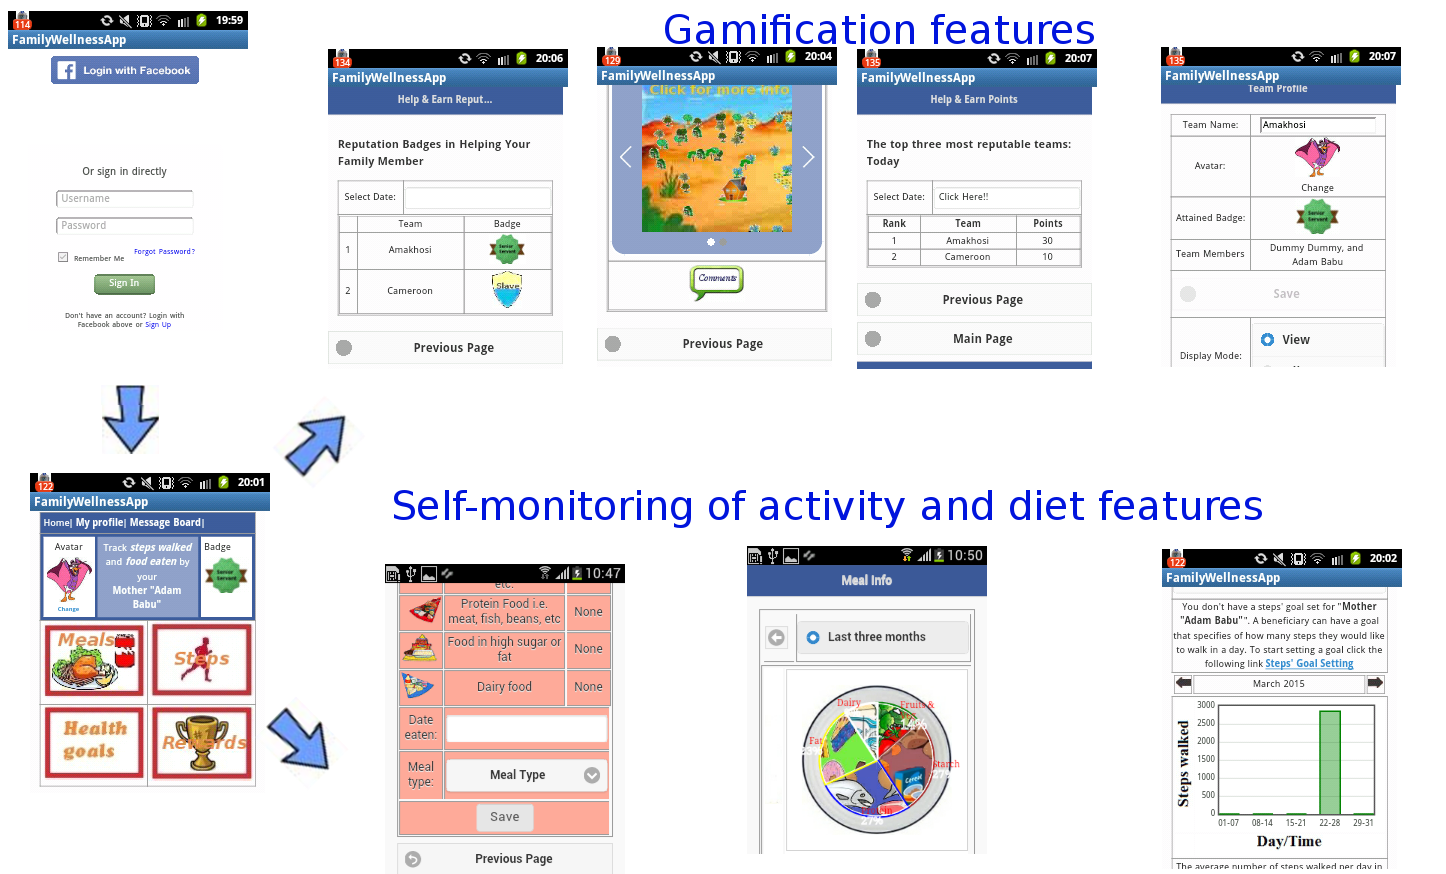
\includegraphics[width=0.8\textwidth]{Figures/Version2/Prototype2Screenshots.png}
    \rule{35em}{0.5pt}
  \caption{Sample screen-shots of the second prototype}
  \label{figure:prototype_2_screens}
\end{figure}

These rules were just arbitrary. The objective was to design challenges with an objective of increasing engagement between intermediaries and beneficiaries when the two users negotiate for interaction with the app.
\section{Prototype Evaluation Description}
The plan in evaluation was to recruit another group of participants. The NGO facilitated access to a group which resided in another side of Philippi where evaluation of the first prototype was conducted. The recruitment was facilitated by the same NGO in Evaluation. But the plan didn't materialize as the NGO advised that we try to look for a different group because the group they were working with expressed concerns regarding safety issues after they heard that they were going to be given phones to use throughout the evaluation period. The NGO was concerned of safety of researchers since rumour had spread throughout the community that someone is going to bring phones to that area. This poses risks to both prospective participants and the researcher. In response to that, this plan was revised and the researcher found another township called Langa, which was a bit smaller and more central township, safer than Philippi.

A research facilitator who is a resident of Langa helped with the recruitment process. This time the recruitment criteria were more stringent compared to the previous evaluation. One of the criteria was to have intermediaries that cohabit or live nearby the beneficiaries. Preference was given to school going children as there were more likely to be interested in gamification. A total of nine adult participants were recruited for the study. The distribution between male and female was three(3) and six(6) respectively. Their average age was 49.3 years old (SD=7.9 years). Each adult participants brought one intermediary participant and formed a pair. The distribution of intermediary participants by gender was 3 males and 6 females. The mean age of these intermediary participants was 14 years old (SD=4.3).  Eight adults  were relatives/familial related to intermediary participants while the remaining adult was just a tenant of her intermediaries' grandmother. Eight intermediary participants were school-going children.
log out
Prior to commencement of the study, both beneficiary and intermediary participants were given information about the study. Participants were informed that the study's cellphone will be collecting their information related to usage of the app, step walked,  and diet and this information will transferred to the researcher's computer at University of Cape Town. All participants who were not minors signed informed consent forms while minors signed assents forms that were also signed by their respective guardians/parents.

Once consent and assent forms were signed, one day was allocated to train intermediary participants on use to use the app. After the training each pair was provided with an one android phone ((Samsung
GT-S5300) that contained two native app. The first app was a pedometer which was not displaying any useful information apart from raw steps' data. The pedometer task was to send these steps to a server so that they can be presented  and viewed in a better format through a web application. The second app provided a link to the web application so that users don't have to type a URL every time they needed to access the web app.

In order to encourage participation, each beneficiary participant received ZAR 40 worth of airtime four times in a period of three weeks (ZAR 160 in total). To encourage participation of intermediary participants, each pair was credited 300MB of data to use on the Android phone as it was expected that intermediaries would borrow phones to access other things on the internet that are beyond prescribed uses.

I left the app in the field for three weeks before conducting an evaluation. After three weeks I conducted the evaluation which is described on the next sub-section.
\section{Prototype Evaluation Methods}
The evaluation relied in two approaches which are collecting user logs and interviews. In interviews, all respondents were familiar/comfortable with English, therefore, interviews were conducted in English. A total of three(3) intermediary participants, and five(5) intermediary participants were interviewed. These are the only participants that I could reach to during the time of interviews. These were short interviews which lasted up to 15 minutes for one person. 
\section{Findings}
The key findings were based on social factors and motivational strategies that influenced usage of the app. Some of the findings from this chapter together with findings from the previous chapter (Chapter \ref{prototype1chapter}) have also appeared in a conference paper that I co-authored \citep{katule2016leveraging}.
\subsection{The Role of a Familial Relationship in the Intervention}
As it was observed in the previous chapter (Chapter \ref{prototype1chapter}), a parent/child relationship may be important in implementation of such an intervention. In this case, a prior social relationship was also very important. Intermediaries that were working with their parents were eager to support their parents because they cared about them. 

Usage of each pair  was clustered its respective relationship type as shown on Figure \ref{figure:relation}. There were three three types of relationships:parent-intermediary, relative-intermediary, and not related , with 4, 3, and 1 number of pairs respectively. Usage on each relationship type was measured through three dimensions: (1)~the average number of days per pair; (2)~the average number of sessions per pair; and (3)~the average number of clicks per pair. More usage was observed on pairs with relationship of type parent-intermediary. 
\begin{figure}[htbp]
  \centering
    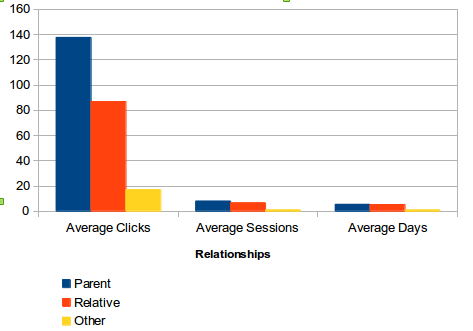
\includegraphics[width=0.6\textwidth]{Figures/relationships.png}
    \rule{35em}{0.5pt}
  \caption{Usage in three groups of relationships\citep{katule2016leveraging}}
  \label{figure:relation}
\end{figure}
In the case of parent-intermediary, or relative-intermediary relationships, negotiation for interaction that initiated by beneficiary users was more possible because of the nature of the prior relationship. For instance the following two scenarios, requests from beneficiaries where always successful most of the time. For instance, \textbf{Zandiwe}, \emph{a beneficiary user, a woman aged 50 years old}, she was working with her sister daughter. Another case was shared by  \textbf{Lulama}, \emph{an intermediary user, a girl aged 20 years old} who was working with her mother, \textbf{Nokanyo}, \emph{aged 57 years old}. 

\userquote{\textbf{Zandiwe}, a beneficiary} {``I used to call Lindiwe [an intermediary is aged 16 years of age] like `Lindiwe there is something that I don't understand'. Or I call her the day before when I walk for a long, I call her to come and help me some way somehow.''}

\userquote{\textbf{Lulama}, an intermediary} {``My mother was the one who was pushing me, let’s do it, let’s do it. And we spent more time together. But we are always together around that time I do the app at around o'clock at night. So we talk more than before because she would ask `How am I doing on this?'''}

There were scenarios of whereby a beneficiary user could request assistance at the time where an intermediary was either resting or occupied by other activities or felt that there was no urgency in fulfilling  such a request. In such a scenario, a social relationship still had to play a role in motivating intermediaries to immediately attend to those requests.

Also for a parent-child relationship,  intermediaries demonstrated sense of being co-owners of the information from the system. For instance, Lulama, used the terms ``we'' or ``our'' repeatedly to describe actions that needed to be carried out by her beneficiary user as actions that needed to be carried out by both of them.
  
\userquote{\textbf{Lulama}, an intermediary} {``When I saw the garden I was like yeah, our garden is looking beautiful. Lets do more. Lets take more steps. Lets eat more veges, because it is the veges and fruits that are important.''}

In addition, intermediaries from pairs with a prior social relationship had more authority in persuading their beneficiaries to do something in order to win. And it was not solely for winning purposes as they cared for health of the people they were helping. This phenomenon was observed in two pairs with the following excerpts.

\userquote{\textbf{Lulama}, an intermediary} {``I am helping her so it [The app] has to mean a lot to me. I am helping her (Nokhanyo) because she doesn't know anything. She is like `What is this?'. This is how you do this. She is like `ooh okay' So it [The app] means a lot to me because I am helping someone I care about.''}

\userquote{\textbf{Nokhanyo}, a beneficiary user} {``Sometimes she used to shout at me. `No no you didn't eat that thing. Tell me what you ate in the morning. I saw you eating this. It seems there is nothing for fruits, peanuts. You must remind me to check you!'''}

\userquote{\textbf{Lwazi} (an intermediary, a boy aged 14 years old)}
{``It [The app] was really good because my 
mother was limiting herself on stuff like pies and fat food. I would tell 
her don't eat this don't eat that. She wasn't eating much vegetables but I 
was encouraging her to eat vegetables''}

It was observed that for pairs that didn't have a parent-child relationship, interactions between intermediaries and beneficiaries where lesser or absent except for cases where an intermediary was motivated by access to the intervention's phone or motivation affordances provided by gamification. But in cases where intermediaries where driven by those factors, still there was some form of a prior social relationship that played a role, i.e. relative-intermediary, although it was not as strong as a parent-intermediary relationship. In these cases, of relative-intermediary relationship, even if the intermediary is not motivated by gamification and the phone, they would still provide infrequent help to their beneficiaries.  In one case where there was no relationship between an intermediary and beneficiary, even the infrequent help was not available i.e. in the case \textbf{Anele} (a beneficiary user, a 47 year old woman, who was working with the granddaughter of her landlord, hence, they were not related. Anele mentioned that every time she passed her request to be helped, her intermediary claimed to be busy and kept on procrastinating by saying they will do it the next day and when that day comes it was the same thing. 

Therefore, a familial relationship played an important role in mediating motivation of some intermediaries to help. 
\subsection{Sources of Motivation for the two Sets of Users}
In cases were both users of a pair were motivated to use the app and there was a prior social relationship between them, then a pair tended to interact in a more playful manner which brought the two users closer compared to before using the app. This happened in  when an intermediary was reporting back the information to a beneficiary user.  This made the interaction between an intermediary and beneficiary to be more enjoyable and less tense. These narration from participants describe how the interaction  between an intermediary and beneficiary was enjoyable, when the two users were engaging with the app.

\userquote{\textbf{Zandiwe}, a beneficiary} {` When she got time, when she is done with her homework she comes and sees the app. And then laughs at me like `Yo yo yo [An interjection for Xhosa speakers to express the feeling of amazement by something] you can walk yo yo yo', like `you walked a lot today' and what what [She was implying to other words said by Lindiwe]''}

In that excerpt above, Lindiwe showed excitement upon seeing steps walked by Zandiwe. Also Nokanyo mentioned how they laugh when she interacts with her daughter when they are exchanging information retrieved from the app. This playful environment fostered relatedness and made it easier for the two users from a pair to continue engaging with the app. 

However in engaging with the app, intermediaries and beneficiaries had different motivational goals. Intermediaries were interested in pursuing a steps or diet goal in order to achieve rewards in gamification. While for beneficiaries, their primary goal was to achieve more steps for the purpose of informal comparisons with others or for instrumental value to their health. These different sources of motivations are further expanded below.
\subsubsection{Sources of Motivation in Beneficiaries}
One of the factors that played a role in motivating beneficiaries was informal comparison of steps/diet. In the app there was no feature that supported direct comparison of steps or diet. Instead, beneficiary participants who knew each other they implicitly formed a social support group. In this support group, they interacted with each other through either face to face meetings or an SMS/a phone call. These interactions were centred around comparison of steps or diet among each other. 

\userquote{\textbf{Zandiwe}, a beneficiary} {``We [with Nokanyo] were talking about what we ate. Like Tuesday I phone Nokanyo to ask her `Did you eat a lot'. She said `not today' But she said she ate a lot the day before. It was Monday.''}

These kinds of social comparisons led to competitions between beneficiary participants. Competition was a  consequence of how the app was existing social context and not an intended goal of design as they happened beyond the app context.  Some beneficiary set their target or goals in order to beat others within a social support group. These beneficiary participants were always curious about how other were doing within their support group.
 
\userquote{\textbf{Lulama}, an intermediary user} {``She [Nokhanyo] would ask `I wonder how so and so is doing'. She would ask them when she sees them. She wouldn't ask on the app ''}

\userquote{\textbf{Ndileka} (beneficiary user), 35 years old woman}
{`` I think I was in competition with steps [She is chuckling]. Because others would have said ooh I have walked, maybe we look at the thing to say let’s 1900 steps. And for me I will say no, tomorrow I need to walk more than her because she walked 1900 steps. Then I need to walk 2500 steps''} 

Also some beneficiaries got interested to some of the gamification features after \emph{proximate translation by beneficiary users}. Therefore, intermediaries needed interpretation of what is going on in gamification in order for them to understand it.

\userquote{\textbf{Lulama}, an intermediary} {``She [Nokhanyo] saw the garden. The
first day she saw just the house and brownish. She
is like `What is this'. I told her. She said `Aha! [Expressing
dissatisfaction]. It must look green and healthy'. And then
she saw the garden again and said `It is looking good.'''}  

\userquote{\textbf{Lwazi}, an intermediary} {``She [His mother] doesn't understand the app. I just tell her that people are having ones twos threes (on the scoreboard and badges) and she laughs''} 

Therefore, the most motivating factors for beneficiaries were steps feedback and comparison of steps with others. 
\subsubsection{Sources of Motivation in Intermediaries}
There are several factors that motivated intermediaries to use the app, apart a prior social rapport. Factors that manifested in participants' responses include gamification features, effect of intervention's phones, and self-monitoring of steps. Some intermediaries nudged their beneficiary
users to do more in steps or to eat healthy, so that their pairs would win rewards offered by gamified elements of the web app. The extent of nudging was evident in pairs with parent-intermediary relationship. Gamification features such as badges and scoreboard mediated competition between intermediaries.

\userquote{\textbf{Lwazi}, an intermediary}
{``The app challenged me to compete [with others] because there was this lady I think it was Lulama. She was getting points and I was really stressed out because she was reaching the amount I was getting so I was pushing hard to get there. But now I am second. If I was using the app so much I was going to be number one but I am not using the app so much because my mother is not putting her sim card on the phone....It the same like a battle, you are battling with other people. So you must be on your toes with the app and see what is going on with your family''}

Intermediaries were able to interpret some of the intentional persuasive strategies for instance the concept of using the size of the fish in relation to recording of diet. For instance Lwazi was asked what was the size of fish in his tank and his response was as follows, \emph{``They were medium sized because I wasn't really feeding them.''}. By not feeding them he implied that he wasn't not doing enough in recording of meals eaten by his mother. This an example of a connection that was made between playful interfaces and actual health self-monitoring behaviours. But there were also other unintentional persuasive effects resulted from SMS reminders. In one context, three participants (one intermediary and two beneficiaries) were convinced that messages were sent by the researcher. These messages were tailored with participants names and they were auto generated. Therefore, these participants perceived them as the researcher was following their performance and was trying to encourage them. For instance, Nokhanyo, every time she received a message she would call her daughter to come and see and tell that it is coming from so and so (mentioning the name of the researcher). This caused Lulama to panic thinking that there is something she did wrong whenever she heard her mother call her about a received SMS. In a different scenario, Lwazi thought that messages were sent by other participants through a message board that was on the app. Therefore, he passed these reminders to his mother telling her that people are saying to us about eating healthy and the mother was always responding with a laughter. But Lwazi used the same messages to encourage his mother to walk more steps and eat healthy.  

Apart from gamification features, a phone had an effect in motivating intermediaries to participate especially the ones that had a prior social relationship with their beneficiaries. Intermediaries were involved in tasks that were non-prescribed in the course of carrying out tasks that within prescribed use. For instance two intermediaries aged 10 and 14 had installed games in intervention's phones that were possessed by their parents. The following is a case of an intermediary who lived a distance from a beneficiary but she came all the way to use the phone and to also interact with gamification.  

\userquote{\textbf{Zandiwe}, a beneficiary} {``Lindiwe likes the phone too much. She is always here after school. She lives with my sister on the other side and she comes here everyday. Sometimes I call her to come. We are closer than before. We always talk about the app while other people (relatives) are around. These people also got interested''} 

\userquote{\textbf{Dlamini}, a beneficiary, man aged 72 years old} {``''} 

There was also the novelty effect from the self-monitoring tasks (diet's pie chart and steps' bar chart ). Some intermediaries got excited to see visualization of information about people they cared about. For instance one intermediary aged 10 years old mentioned that steps were the most interesting out of all features. 

\subsection{Perceived Value in Using the Prototype}
Beneficiaries mentioned that they had gained value inform of knowledge and their health.

\userquote{\textbf{Zandiwe}, a beneficiary} {``There are a lot of things I didn't know I now know, like how to eat. I know walking is very important. Because you know I am fat. When I stay on the bed the whole day my blood doesn't circulate.''} 

\userquote{\textbf{Ndileka}, a beneficiary} {``The app helped me because sometimes you don't realize you eat more carbohydrate than fruits. You just eat bread but you don't know that bread is carbohydrate. So when it says large amount of carbohydrate, so you know I am eating large amount of carbohydrate. You think now I must eat more fruits than meat or less meat. So for me automatically it helped me to think that I need to eat large amount of fruits.''}

The case of Ndileka above is referred to as cognitive dissonance. This is why self-monitoring is so important because it shows an individual if there is a discrepancy between their beliefs and their actions. Cognitive dissonance supports individuals to restore consistence between beliefs and actions\citep{Oinas-kukkonen:psd}

Intermediaries who engaged with the app also reported that their beneficiaries had have become more knowledgeable about living healthy. 
\section{Discussion}
Existing social rapport is important for this kind of intervention. Social rapport creates a conducive atmosphere for using different strategies to motivate both intermediaries and beneficiaries. Social rapport and external motivation sources go in parallel and may depend on each other. For instance,  external sources motivation such as phone effect and gamification can enhance an existing familial relationship as it is suggested on the findings. Perceived relatedness between family member had increased. In addition, familial relationship created an opportunity of utilizing young family members as persuaders for behaviour change. These intermediaries can create intents to persuade. This approach relied on social rapport within a household which can be much stronger than a social rapport with an individual who is not a family member. This approach is different from existing approaches in ICTD context.  For instance there is a project in India that leveraged trust between community health workers and expectant mothers for  persuasion~\citep{ramachandran2010mobile,ramachandran2010research}, and this trust was built based on persuasive information that community health workers (CHWs) possessed on their phones. Therefore, the prior social rapport is relatively weak, and the  influence of these CHWs can be limited to infrequent visits, and much of the persuasive strategy relies on the messages possessed by CHWs \citep{katule2016leveraging}.  

Apart from the prerequisite of a prior social relationship, motivation strategies are important as they strengthen on what already the social relationship  that exists. Intermediaries and beneficiaries had different motivational needs when engaging with the app. Intermediaries focused on gamification part as their primary objective. Steps and meals were secondary objectives since they were some how linked to the gamification part. Beneficiaries considered steps and meals as their primary objective. Intermediaries competed in points on the leader board but beneficiaries competed on the number of steps walked or healthy meals. Therefore, in this context there are two sets of users that need to be persuaded differently since they have different objectives. Motivational strategies for the two users need to be examined separately, and a designer has to come up with an optimal strategy that will combine motivational strategies for the two groups. An understanding of context is crucial and this has been emphasized by~\citep{Oinas-kukkonen:psd, Oinas-Kukkonen:foundation}. 

If we delve into the sources of motivation by intermediary users, one can see motivation is of twofold. The first dimension has an aspect ego-involved and the second dimension has an aspect of task mastery climate. The ego involved aspect is exhibited through review of statements by the following two intermediary users (\textbf{Lwazi} and \textbf{Lulama}). Let's refer to one excerpt by \textbf{Lwazi} which mentioned about being stressed out upon seeing others coming to the top of the leaderboard. If one interprets that statement through the view of internalization of behaviour regulation discussed on the literature review chapter, the above scenario promotes introjected regulation of where there is ego involved; hence usage in such context may appear to be influenced by attempts to outperform others. Also the same emphasis on outperforming others is exhibited by \textbf{Lulama}. So the aforementioned comparisons were respect to the leaderboard. The aspect of motivation that focuses on problem solving or task mastery is demonstrated on the excerpt by \textbf{Lulama} of where she was explaining the discussion with her mother (\textbf{Nukhanyo}) about the meaning of the garden. From this conversation, \textbf{Nukhanyo} emphasizes that their garden must look green. Also in some of \textbf{Lulama}'s conversations, she kept on emphasizing by making their garden green by eating more vegetables. Therefore, both \textbf{Lulama} and \textbf{Nukhanyo} are able to make a connection of what they need to do in order master the task of making the garden greener. 

The two aspects of motivation of which one promotes ego-involved climate, and the other promotes task-mastery climate are expanded on, findings of the next chapter (Chapter \ref{discussionchapter}), the overall discussion chapter (Chapter \ref{summativeevalchapter}) which attempts to collate the findings from all three evaluations in order to broaden the discussion about the implication of this specific finding to the design of gamification.
 
\begin{flushright}
\end{flushright}
